\chapter{Indledning}

\section{Baggrund}
Den demografiske udvikling er en kendt og omtalt faktor i store dele af verden og  det danske samfundet er også under pres. Vi bliver flere ældre og færre erhvervsaktive\cite{KL}. Udviklingen gør, at der er færre i den arbejdsdygtige aldre til at forsørge de flere udenfor denne aldre. På sigt vil det skabe store problemer, særligt indenfor sundheds- og plejesektoren både samfundsøkonomisk og ressourcemæssigt. Med disse demografiske samt økonomiske udfordringer Danmark står overfor, er det nødvendigt at tænke i andre baner. Digitaliseringsstyrelsen mener, at sundhed skal leveres på nye mere smarte og teknologiske måder\cite{Digst}.    

Telemedicin er derfor for alvor kommet på dagsorden hos regeringen, regionerne og kommunerne. I 2012 udarbejdede disse parter en ambitiøs national handlingsplan for udbredelsen af telemedicin i Danmark\cite{Digst}, \cite{NationalH}.\\
Digitaliseringsstyrelsen er ved at lave en ny fællesoffentlig digitaliseringsstrategi frem mod 2020, hvor datadeling, datasikkerhed og it-infrastruktur er temaer\cite{digst1}. Denne strategi skal understøtte de teknologiske muligheder for smartere og mere sikker deling af data mellem borger og offentlige sektor\cite{digst2}.\\
Kommunernes strategi er fokuseret bredere - nemlig på telesundhed og ikke telemedicin.

Telemedicin er en underbegreb indenfor telesundhed, hvor telesundhed indgår i det overordnede begreb velfærdsteknologi\cite{KLs}. Forholdet mellem de tre begreber er illustreret i figur 1.3. 

\begin{figure}[H]
	\centering
		\caption{Forholdet mellem velfærdsteknologi, telesundhed og telemedicin\cite{KLs}.}
	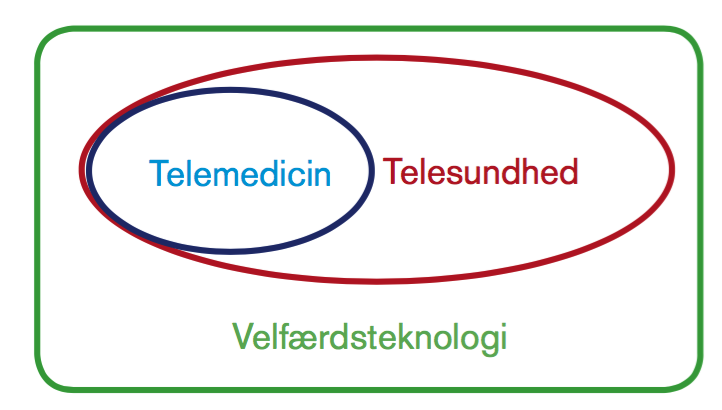
\includegraphics[width=0.6\textwidth]{Figurer/Snip20160426_6}
\end{figure}

I "Kommunernes strategi for telesundhed"\ defineres telesundhed som brugen af informations- og kommunikationsteknologi til at understøtte forebyggende, behandlende eller rehabiliterende aktiviteter over afstand\cite{KLs}. Hvorimod telemedicin er mere fokuseret på selve diagnosen og behandlingen, som borgeren har behov for. Telesundhed fokuserer på borgernes helbred, inden de bliver patienter\cite{KLs}\cite{sundhed}.

Kommunernes mål med telesundhed er at gøre borgerne mere selvstændige, uafhængige af tid og sted og øge deres følelse af at kunne mestre eget liv. Telesundhed skal som minimum kunne levere ydelserne af samme kvalitet som før\cite{KLs}.

Kommunerne mener, at telesundhedsløsningerne har et stort potentiale og kan være med til at varetage forskellige kommunale opgaver. I hjemmeplejen har man i flere kommuner blandt andet Viborg\cite{viborg}, Halsnæs\cite{hals} og Favrskov forsøgt sig med virtuel hjemmepleje. 

I 2015 startede Favrskov kommune et projekt op omkring telesundhed, virtuel hjemmepleje. Projektet forløber i to dele, hvor den første del er et pilotprojekt, hvor formålet er at opnå erfaringer, identificere ydelsestyper samt at kunne udarbejde en businesscase for virtuel hjemmepleje i Favrskov kommune. Anden del af projektet er den brede udrulning i hele kommunen. Hele projektets mål er at erstatte fysisk tilstedeværelse hos borgeren, hvor ydelsen blot indebærer påmindelse eller støtte, med videokonference. Borgerens sikkerhed og tryghed skal bevares, samtidig med at kommunen opnår en effektivisering\cite{projektplan}. 

Projektet startede op på baggrund af et kørende projekt i Lyngby-Tårbæk, som havde til formål at screene KOL patienter. Lyngby-Tårbæk benyttede Appinux's telemedicinske platform og på baggrund af Lyngby-Tårbæk's erfaringer, valgte Favrskov kommune Appinux's telemedicinske løsning \textbf{(Bilag ? mail fra Karin)}.

\section{Formål}
Konsulenthuset, Netplan Care og Favrskov Kommune er i gang med et innovationssamarbejde om udviklingen af en kommunal digital velfærdsteknologisk sundhedsstrategi for telesundhed. Som et led i denne sundhedsstrategi har sundhedsteknologistuderende fra Aarhus Ingeniørhøjskole udarbejdet denne mini-MTV, der har til formål at vurdere brugen af Appinux's telemedicinske løsning i Farvskov kommune, hvor ydelsen påmindelse om medicin- og fødeindtag leveres via videokonference. Vurderingen vil tage udgangspunkt i teknologien omkring Appinux's telemedicinske løsning, de borgmæssige- og organisatoriske betydninger samt de økonomiske omkostninger ved indførelsen af virtuel hjemmepleje i Farvskov kommune.  

\section{Fokuserede spørgsmål}
De opstillede fokuserede spørgsmål er dem, der ønskes besvares gennem denne mini-MTV. 

\begin{itemize}
	\item Hvordan fungerer Appinux-løsningen med videokonference i Favrskov Kommune? Spørgsmålet søges besvaret med udgangspunkt i følgende punkter:
	\begin{itemize}
	\item Sikkerhedskrav
	\item Dækning %(video-conferencing, kodeks mm)
	\item Kompatibilitet 
\end{itemize}
\end{itemize}

\begin{itemize}
	\item Hvilke borgermæssige betydninger er der ved implementering og drift af virtuel hjemmepleje med videokonference i Favrskov Kommune? Spørgsmålet søges besvaret med udgangspunkt i følgende punkter:
	\begin{itemize}
	\item Tilfredshed
	\item Borgeraccept
	\item Tryghed
\end{itemize}
\end{itemize}

\begin{itemize}
	\item Hvilke organisatoriske betydninger er der ved implementering og drift af virtuel hjemmepleje med videokonference sammenlignet med konventionel fysisk hjemmepleje i Favrskov Kommune? Spørgsmålet søges besvaret med udgangspunkt i følgende punkter:
	\begin{itemize}
	\item Forskel i medarbejdernes arbejdsgange før/efter virtuel hjemmepleje
	\item Medarbejdernes reaktion
\end{itemize}
\end{itemize}


\begin{itemize}
	\item Hvilke økonomiske omkostninger er der ved implementering og drift af virtuel hjemmepleje med videokonference sammenlignet med konventionel fysisk hjemmepleje i Favrskov Kommune?
\end{itemize}

